\documentclass{standalone}
\usepackage{tikz}
\usetikzlibrary{patterns, positioning}


\begin{document}
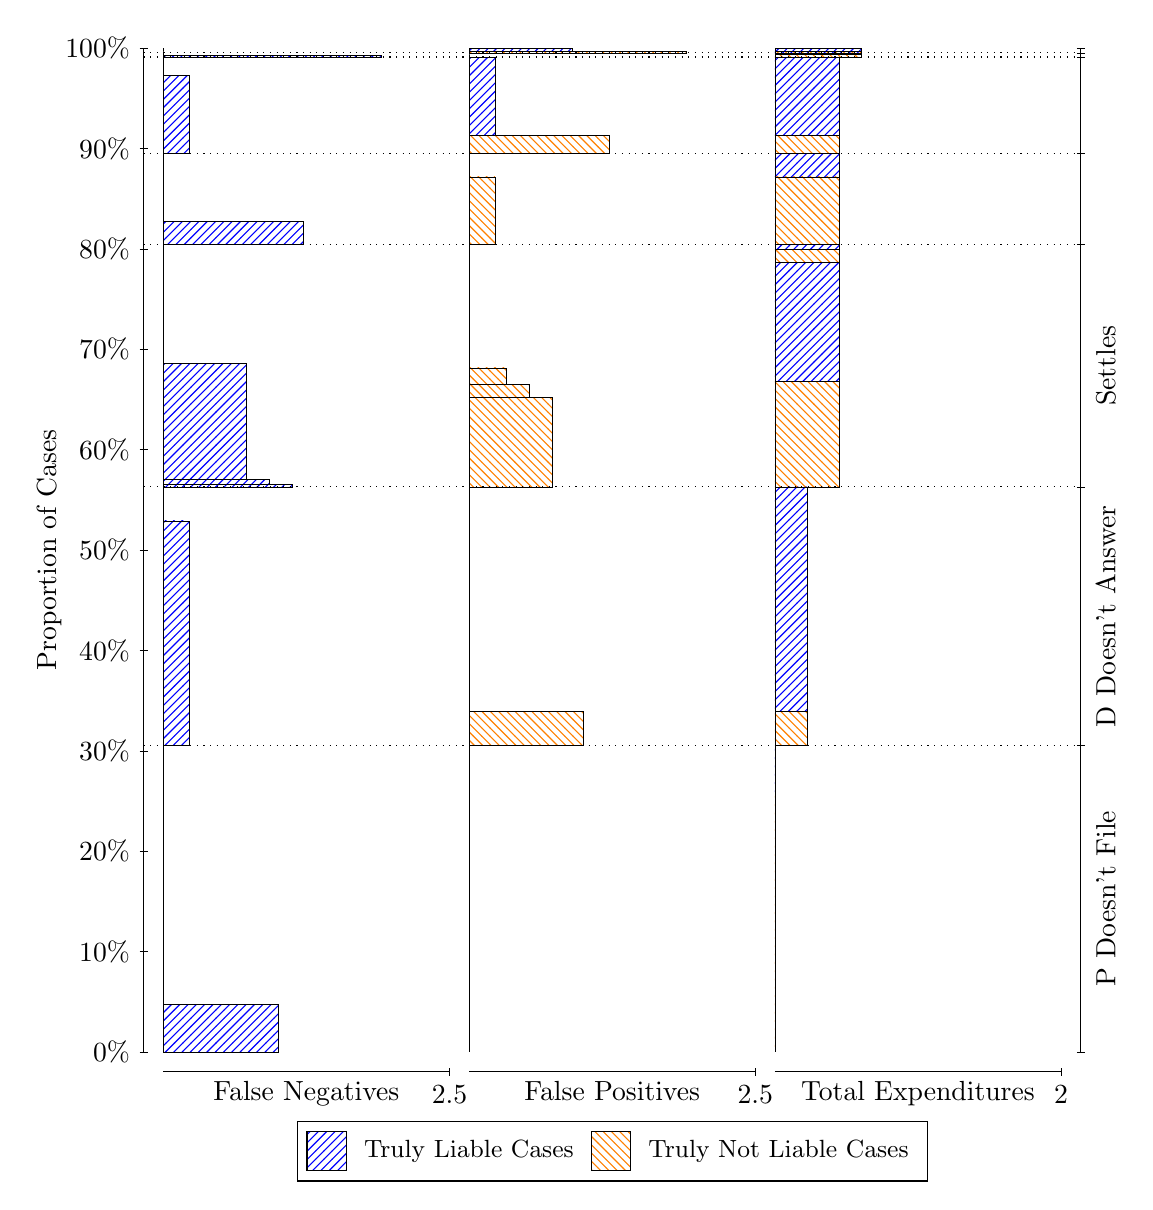
\begin{tikzpicture}
\draw[black, very thin] (1.5,1.75) -- (1.5,14.5);
\node[rotate=90, text=black, anchor=center] at (0.3, 8.125) {Proportion of Cases};
\draw[black, very thin] (1.45,1.75) -- (1.55,1.75);
\node[text=black, anchor=east] at (1.45, 1.75) {0\%};
\draw[black, very thin] (1.45,3.025) -- (1.55,3.025);
\node[text=black, anchor=east] at (1.45, 3.025) {10\%};
\draw[black, very thin] (1.45,4.3) -- (1.55,4.3);
\node[text=black, anchor=east] at (1.45, 4.3) {20\%};
\draw[black, very thin] (1.45,5.575) -- (1.55,5.575);
\node[text=black, anchor=east] at (1.45, 5.575) {30\%};
\draw[black, very thin] (1.45,6.85) -- (1.55,6.85);
\node[text=black, anchor=east] at (1.45, 6.85) {40\%};
\draw[black, very thin] (1.45,8.125) -- (1.55,8.125);
\node[text=black, anchor=east] at (1.45, 8.125) {50\%};
\draw[black, very thin] (1.45,9.4) -- (1.55,9.4);
\node[text=black, anchor=east] at (1.45, 9.4) {60\%};
\draw[black, very thin] (1.45,10.675) -- (1.55,10.675);
\node[text=black, anchor=east] at (1.45, 10.675) {70\%};
\draw[black, very thin] (1.45,11.95) -- (1.55,11.95);
\node[text=black, anchor=east] at (1.45, 11.95) {80\%};
\draw[black, very thin] (1.45,13.225) -- (1.55,13.225);
\node[text=black, anchor=east] at (1.45, 13.225) {90\%};
\draw[black, very thin] (1.45,14.5) -- (1.55,14.5);
\node[text=black, anchor=east] at (1.45, 14.5) {100\%};

\draw[black, very thin] (13.4,1.75) -- (13.4,14.5);
\draw[black, very thin] (13.35,1.75) -- (13.45,1.75);
\node[anchor=west] at (13.35, 1.75) {};
\draw[black, very thin] (13.35,5.6409) -- (13.45,5.6409);
\node[anchor=west] at (13.35, 5.6409) {};
\draw[black, very thin] (13.35,8.9278) -- (13.45,8.9278);
\node[anchor=west] at (13.35, 8.9278) {};
\draw[black, very thin] (13.35,12.004) -- (13.45,12.004);
\node[anchor=west] at (13.35, 12.004) {};
\draw[black, very thin] (13.35,13.158) -- (13.45,13.158);
\node[anchor=west] at (13.35, 13.158) {};
\draw[black, very thin] (13.35,14.386) -- (13.45,14.386);
\node[anchor=west] at (13.35, 14.386) {};
\draw[black, very thin] (13.35,14.438) -- (13.45,14.438);
\node[anchor=west] at (13.35, 14.438) {};
\draw[black, very thin] (13.35,14.5) -- (13.45,14.5);
\node[anchor=west] at (13.35, 14.5) {};

\draw[black, very thin, pattern color=blue, pattern=north east lines] (1.75,1.75) rectangle (3.2033,2.35);
\draw[black, very thin, pattern color=orange, pattern=north west lines] (1.75,2.35) rectangle (1.75,5.6409);
\draw[black, very thin, pattern color=blue, pattern=north east lines] (1.75,5.6409) rectangle (2.077,8.4946);
\draw[black, very thin, pattern color=orange, pattern=north west lines] (1.75,8.4946) rectangle (1.75,8.9278);
\draw[black, very thin, pattern color=blue, pattern=north east lines] (1.75,8.9278) rectangle (3.385,8.9567);
\draw[black, very thin, pattern color=blue, pattern=north east lines] (1.75,8.9567) rectangle (3.0943,9.0204);
\draw[black, very thin, pattern color=blue, pattern=north east lines] (1.75,9.0204) rectangle (2.8037,10.495);
\draw[black, very thin, pattern color=orange, pattern=north west lines] (1.75,10.495) rectangle (1.75,12.004);
\draw[black, very thin, pattern color=blue, pattern=north east lines] (1.75,12.004) rectangle (3.5303,12.299);
\draw[black, very thin, pattern color=orange, pattern=north west lines] (1.75,12.299) rectangle (1.75,13.158);
\draw[black, very thin, pattern color=blue, pattern=north east lines] (1.75,13.158) rectangle (2.077,14.155);
\draw[black, very thin, pattern color=orange, pattern=north west lines] (1.75,14.155) rectangle (1.75,14.386);
\draw[black, very thin, pattern color=blue, pattern=north east lines] (1.75,14.386) rectangle (4.5113,14.405);
\draw[black, very thin, pattern color=orange, pattern=north west lines] (1.75,14.405) rectangle (1.75,14.438);
\draw[black, very thin, pattern color=orange, pattern=north west lines] (1.75,14.438) rectangle (1.75,14.457);
\draw[black, very thin, pattern color=blue, pattern=north east lines] (1.75,14.457) rectangle (1.75,14.5);
\draw[black, very thin, pattern color=orange, pattern=north west lines] (5.6333,1.75) rectangle (5.6333,5.0409);
\draw[black, very thin, pattern color=blue, pattern=north east lines] (5.6333,5.0409) rectangle (5.6333,5.6409);
\draw[black, very thin, pattern color=orange, pattern=north west lines] (5.6333,5.6409) rectangle (7.0867,6.0742);
\draw[black, very thin, pattern color=blue, pattern=north east lines] (5.6333,6.0742) rectangle (5.6333,8.9278);
\draw[black, very thin, pattern color=orange, pattern=north west lines] (5.6333,8.9278) rectangle (6.687,10.061);
\draw[black, very thin, pattern color=orange, pattern=north west lines] (5.6333,10.061) rectangle (6.3963,10.228);
\draw[black, very thin, pattern color=orange, pattern=north west lines] (5.6333,10.228) rectangle (6.1057,10.437);
\draw[black, very thin, pattern color=blue, pattern=north east lines] (5.6333,10.437) rectangle (5.6333,12.004);
\draw[black, very thin, pattern color=orange, pattern=north west lines] (5.6333,12.004) rectangle (5.9603,12.863);
\draw[black, very thin, pattern color=blue, pattern=north east lines] (5.6333,12.863) rectangle (5.6333,13.158);
\draw[black, very thin, pattern color=orange, pattern=north west lines] (5.6333,13.158) rectangle (7.4137,13.389);
\draw[black, very thin, pattern color=blue, pattern=north east lines] (5.6333,13.389) rectangle (5.9603,14.386);
\draw[black, very thin, pattern color=orange, pattern=north west lines] (5.6333,14.386) rectangle (5.6333,14.419);
\draw[black, very thin, pattern color=blue, pattern=north east lines] (5.6333,14.419) rectangle (5.6333,14.438);
\draw[black, very thin, pattern color=orange, pattern=north west lines] (5.6333,14.438) rectangle (8.3947,14.457);
\draw[black, very thin, pattern color=blue, pattern=north east lines] (5.6333,14.457) rectangle (6.9413,14.5);
\draw[black, very thin, pattern color=orange, pattern=north west lines] (9.5167,1.75) rectangle (9.5167,5.0409);
\draw[black, very thin, pattern color=blue, pattern=north east lines] (9.5167,5.0409) rectangle (9.5167,5.6409);
\draw[black, very thin, pattern color=orange, pattern=north west lines] (9.5167,5.6409) rectangle (9.9254,6.0742);
\draw[black, very thin, pattern color=blue, pattern=north east lines] (9.5167,6.0742) rectangle (9.9254,8.9278);
\draw[black, very thin, pattern color=orange, pattern=north west lines] (9.5167,8.9278) rectangle (10.334,10.269);
\draw[black, very thin, pattern color=blue, pattern=north east lines] (9.5167,10.269) rectangle (10.334,11.773);
\draw[black, very thin, pattern color=orange, pattern=north west lines] (9.5167,11.773) rectangle (10.334,11.941);
\draw[black, very thin, pattern color=blue, pattern=north east lines] (9.5167,11.941) rectangle (10.334,12.004);
\draw[black, very thin, pattern color=orange, pattern=north west lines] (9.5167,12.004) rectangle (10.334,12.863);
\draw[black, very thin, pattern color=blue, pattern=north east lines] (9.5167,12.863) rectangle (10.334,13.158);
\draw[black, very thin, pattern color=orange, pattern=north west lines] (9.5167,13.158) rectangle (10.334,13.389);
\draw[black, very thin, pattern color=blue, pattern=north east lines] (9.5167,13.389) rectangle (10.334,14.386);
\draw[black, very thin, pattern color=orange, pattern=north west lines] (9.5167,14.386) rectangle (10.607,14.419);
\draw[black, very thin, pattern color=blue, pattern=north east lines] (9.5167,14.419) rectangle (10.607,14.438);
\draw[black, very thin, pattern color=orange, pattern=north west lines] (9.5167,14.438) rectangle (10.607,14.457);
\draw[black, very thin, pattern color=blue, pattern=north east lines] (9.5167,14.457) rectangle (10.607,14.5);
\draw[black, dotted] (1.5,5.6409) -- (13.4,5.6409);
\draw[black, dotted] (1.5,8.9278) -- (13.4,8.9278);
\draw[black, dotted] (1.5,12.004) -- (13.4,12.004);
\draw[black, dotted] (1.5,13.158) -- (13.4,13.158);
\draw[black, dotted] (1.5,14.386) -- (13.4,14.386);
\draw[black, dotted] (1.5,14.438) -- (13.4,14.438);
\draw[black, very thin] (1.75,1.5) -- (5.3833,1.5);
\node[text=black, anchor=north] at (3.5667, 1.5) {False Negatives};
\draw[black, very thin] (5.3833,1.45) -- (5.3833,1.55);
\node[text=black, anchor=north] at (5.3833, 1.45) {2.5};

\draw[black, very thin] (5.6333,1.5) -- (9.2667,1.5);
\node[text=black, anchor=north] at (7.45, 1.5) {False Positives};
\draw[black, very thin] (9.2667,1.45) -- (9.2667,1.55);
\node[text=black, anchor=north] at (9.2667, 1.45) {2.5};

\draw[black, very thin] (9.5167,1.5) -- (13.15,1.5);
\node[text=black, anchor=north] at (11.333, 1.5) {Total Expenditures};
\draw[black, very thin] (13.15,1.45) -- (13.15,1.55);
\node[text=black, anchor=north] at (13.15, 1.45) {2};

\node[text=black, centered, rotate=90] at (13.72, 3.6955) {P Doesn't File};
\node[text=black, centered, rotate=90] at (13.72, 7.2844) {D Doesn't Answer};
\node[text=black, centered, rotate=90] at (13.72, 10.466) {Settles};





\draw (7.449999999999999,1.5) node[draw=none] (baseCoordinate) {};
\begin{scope}[align=center]
        \matrix[scale=0.5, draw=black, below=0.5cm of baseCoordinate, nodes={draw}, column sep=0.1cm]{
            \node[rectangle, draw, minimum width=0.5cm, minimum height=0.5cm, pattern color=blue, pattern=north east lines] {}; &
            \node[draw=none, font=\small, text=black] (B) {Truly Liable Cases}; &
            \node[rectangle, draw, minimum width=0.5cm, minimum height=0.5cm, pattern color=orange, pattern=north west lines] {}; &
            \node[draw=none, font=\small, text=black] (B) {Truly Not Liable Cases}; \\
            };
\end{scope}

\end{tikzpicture}
\end{document}